%!TEX program = xelatex
% 完整编译: xelatex -> bibtex -> xelatex -> xelatex
\documentclass[lang=cn,12pt,a4paper,cite=authoryear]{elegantpaper}

\title{数据挖掘课程设计报告}
\author{姓名:姚远\and 学号: 162150109}


%\institute{\href{https://elegantlatex.org/}{Elegant\LaTeX{} 项目组}}

%\version{0.09}
\date{\zhtoday}


% 本文档命令
\usepackage{array}
\usepackage{pythonhighlight}
\usepackage{amsmath,bm}
\usepackage{listings}
\lstset{
    numbers=left,
    framexleftmargin=.5mm,
    frame=shadowbox
}
\usepackage{hyperref}
\hypersetup{hidelinks,
	colorlinks=true,
	allcolors=blue,
	pdfstartview=Fit,
	breaklinks=true}
\usepackage{graphicx}

\newcommand{\ccr}[1]{\makecell{{\color{#1}\rule{1cm}{1cm}}}}

\begin{document}
\maketitle

\section{任务概况}
\subsection{数据集}
本课设数据集来自于 \href{https://www.kaggle.com/competitions/classify-leaves}{Kaggle}, 为树叶分类数据集. 该数据集包含176类不同的树叶, 18353张训练样本(每种树叶至少50个样本, 长尾效应并不明显)以及8800张测试样本. 分辨率皆为 $224 \times 224$. 可以发现这是一个简单的图片分类任务.
\subsection{评测指标}
Kaggle官方直接采用 \href{https://www.kaggle.com/vipulgandhi/how-to-choose-right-metric-for-evaluating-ml-model}{Classification Accuracy} 作为竞赛评测标准. 一般在数据类别均衡的情况下, 模型的acc越高, 说明模型的精度越好. 本数据集由于类别很多, 数据分布较为平均(长尾比约3:1), 因此不考虑通过计算每个类别的recall值来评测模型.
\subsection{解决方案}
事实上这是一个课程网站的project, 该课程是深度学习相关课程, 因此如果你去查看 \href{https://www.kaggle.com/competitions/classify-leaves/code}{Code} 就会发现清一色的 Resnet 与其它深度学习方法.

本课设大致分为传统机器学习和深度学习两种方案来解决问题. \\传统机器学习解决的过程大致包括:
\begin{enumerate}
    \item 训练集验证集划分: 考虑到传统机器学习方法性能较优, 故采用5-Fold Cross Validation, 训练验证比4:1;
    \item 数据预处理: 包括特征提取(SIFT、HOG etc.)、动态聚类(Kmeans)、降维(PCA)等, 将数据转化为统一的向量形式;
    \item 模型分类: 通过采用不同的机器学习分类模型(KNN、SVM etc.)来测试分类效果.
\end{enumerate}
深度学习的过程大致包括:
\begin{enumerate}
    \item 找张GPU: 使用Autodl上的NVIDIA GTX 2080ti(11GB)与校内GPU服务器的NVIDIA RTX A5000(24GB)训练深度学习模型;
    \item 训练集验证集划分: 性能原因, 不考虑使用k-fold, 直接划分. 训练验证比4:1;
    \item 数据预处理: 包括一系列的数据增强(随机翻转、标准化)以及采用跨图片增强(训练过程中体现)的trick: MixUp、CutMix;
    \item 训练验证模型: 对比采用不同的跨图片增强trick训练出来的深度学习模型(resnet及其变种)在验证集上的效果.
\end{enumerate}

\subsection{DummyClassifier}
直接采用DummyClassifier作5折交叉验证, 预测结果为训练样本中出现次数最多的类, 得出最优的acc为0.036.
\section{传统机器学习模型}
事先说明: 本部分所有方法均采用5折交叉验证, 所提到的acc如未说明均为五折平均的acc.
\subsection{特征提取}
\subsubsection{SIFT特征提取}
SIFT(Scale-invariant feature transform)中文名为尺度不变性特征变换, 在传统的CV算法中拥有很高的地位. 作为一个特征点的提取算法, 它对尺度、旋转、关照等变化不敏感, 导致其效果较优.

首先我们有必要弄明白特征点: 对于平滑的区域一般变化不大, 这不是我们关心的地方, 我们关心的是纹理复杂的地方, 例如边缘、点、角之类的区域, 而这些灰度值变换大的地方就是我们要的特征点.

算法的第一步是数据预处理. 由于彩色图是三通道的, 我们需要先将其转化为灰度图, 此时灰度图为单通道, 灰度值应该在0-255之间分布.

算法的第二步是构建多尺度DoG空间. 这里的多尺度代表对不同分辨率的图片作空间构造. 对于单个分辨率的图片, 分别作六次不同方差高斯模糊后的图像:
\begin{equation*}
    \sigma, k\sigma, k^2\sigma, k^3\sigma, k^4\sigma, k^5\sigma.
\end{equation*}

对于特定的方差 $\sigma$, 高斯模糊后的图像的空间灰度函数为:
\begin{equation*}
\begin{aligned}
    G(x_i, y_i, \sigma) &= \frac{1}{2\pi \sigma^2}\exp{\left(-\frac{(x-x_i)^2+(y-y_i)^2}{2\sigma^2}\right)}\\
    L(x, y, \sigma) &= G(x, y, \sigma) * I(x, y).
\end{aligned}
\end{equation*}

然后需要获取高斯差分函数(DoG). 高斯差分图像是某一相同分辨率的相邻图像作差值得出, 然后与原图像 $I(x, y)$ 作卷积得到DoG函数:
\begin{equation*}
\begin{aligned}
    D(x, y, \sigma) &= \left[G(x, y, k\sigma)-G(x, y, \sigma)\right] * I(x, y)\\
    &=L(x, y, k\sigma) - L(x, y, \sigma).
\end{aligned}
\end{equation*}

这样, 对于不同的分辨率, 我们有5个DoG函数. 事实上这就是高斯金字塔表达, 对于不同的尺度(分辨率), 从下到上依次降采样, 长的很像一个金字塔.
\begin{figure}[h]
    \centering
    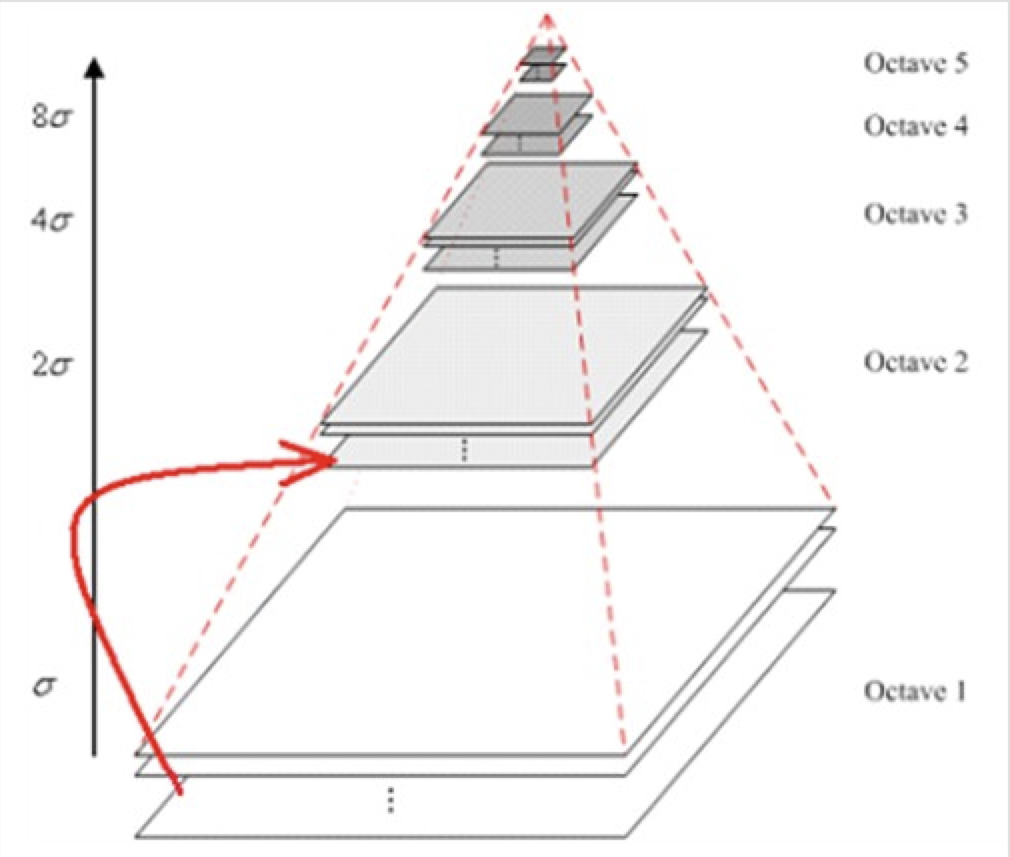
\includegraphics[width=0.5\textwidth]{lateximgs/1.png}
    \caption{高斯金字塔}
    \label{fig:example}
\end{figure}

算法的第三步是极值点检测. 寻找DoG函数的极值点, 最简单的想法是直接和附近点相比较. 在SIFT算法中我们还需要对同一组中上面和下面不同的DoG函数的点相比较, 这样一共需要比较 $8+9\times2=26$ 次, 而对于每组5个DoG函数的情况, 我们只能对中间3个函数进行操作.

然而这种方法找到的点的位置都是在整数空间上的. 换句话说, 这些极值点都是离散的. 因此SIFT算法考虑通过插值法对离散的DoG函数进行曲线拟合, 进一步对方程求偏导, 得到精确的极值点.

此外算法还提到了删除边缘效应的点的概念, 这里不予赘述.

算法的最后一步是产生特征点描述. 上面的过程产生的特征点只有位置信息, 我们需要通过这些特征点附近区域获取特征. 算法在检出的特征点为中心选$16\times16$ 的空间作为特征提取空间, 然后将这些区域均分为 $4 \times 4$ 个子区域. 

对于每个 $4 \times 4$ 的子区域, 计算8个方向的梯度方向直方图. 首先我们计算每个像素的梯度的幅值和方向, 然后对子区域进行统计, 统计8个方向的幅度. (类似HOG的特征提取)

幅度公式:
\begin{equation*}
    m(x, y) = \sqrt{\left(L(x+1, y)-L(x-1, y)\right)^2+\left(L(x, y+1)-L(x, y-1)\right)^2}.
\end{equation*}

方向公式:
\begin{equation*}
    \theta(x, y) = \arctan\left((L(x, y+1)-L(x, y-1))/(L(x+1, y)-L(x-1, y))\right).
\end{equation*}

然后将所有子区域的幅度直方图连接起来, 即可获得特征向量, 其维度为 $4 \times 4 \times 8 = 128$ 维.

\subsubsection{HOG特征提取}
HOG(Histogram of Oriented Gradient)中文名为方向梯度直方图, 相比于晦涩难懂的SIFT, 这个算法更加直接, 直接在原图的基础上产生特征向量. HOG通过计算并统计图像局部区域内的梯度方向直方图(SIFT部分已经介绍过了)来形成特征, 这导致它对图像几何和光学的变化不敏感.

与SIFT算法一样, HOG也需要先将原图片转换为灰度图, 因为HOG提取的是纹理特征, 颜色信息并无作用.

第二步是划分子区域, 在HOG中叫做划分cell, 本课设中每个cell为 $8 \times 8$ 个像素, 且相邻cell不重叠. 然后我们对每个像素计算其梯度幅值和方向, 将所有方向分为9个块, 在每个cell内统计梯度方向直方图.

第三步, 我们需要将多个cell组合成更大的连通块(block), 将block内的所有cell的特征向量串联起来得到HOG的特征描述. 这里相邻的block之间可能重叠. 在更大的范围内统计梯度直方图, 并做归一化处理. 本课设采用L2-norm normalization:
\begin{equation*}
    v = \frac{v}{\sqrt{|v|^2_2+\epsilon^2}}
\end{equation*}

最后, 假设每个block包括 $2 \times 2$ 个cell, 相邻的block之间有1个cell宽度的交集. 那么对于我们分辨率为 $224 \times 224$ 的图片, 所产生的特征向量的维度应该为: $(224/8-1)^2\times9\times4=26244$ 维, 过于庞大. 因此我们先将图片转换为 $128 \times 64$ 分辨率(因为论文就这么搞的), 这样会得到一个 $(128/8-1)\times(64/8-1)\times4\times9=3780$ 维的特征向量, 依旧庞大, 后续会进行降维处理.

\subsection{特征预处理}
\subsubsection{KMeans动态聚类}
聚类分析又称群分析,它是研究对样品或指标进行分类的一种多元统计方法. 聚类分析要使得同一类中的对象之间的相似性比与其他类的对象的相似性更强, 目的在于使同类间对象的同质性最大化和类与类间对象的异质性最大化.

一般地, 聚类分析包括系统聚类和动态聚类. 系统聚类的缺点是每次合并不同类的时候, 结果就已经固定了. 相比系统聚类, 动态聚类法(即KMeans)会根据需求, 动态地调整分类方式.

KMeans聚类方法最简单的表达如下图所示:

\begin{figure}[h]
    \centering
    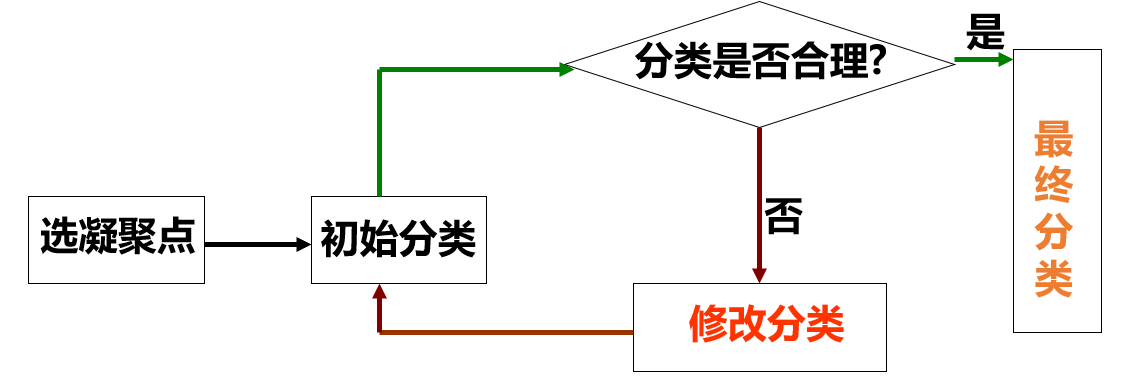
\includegraphics[width=0.5\textwidth]{lateximgs/2.png}
    \caption{KMeans大致过程}
\end{figure}

KMeans常用的一种方法是按批修改法, 它的修改原则是使如下的分类函数逐渐减小:
\begin{equation*}
    l(G_1,\cdots, G_k) = \sum_{i=1}^k \sum_{j=1}^{n_i}(\bm{x}_j^i-\overline{\bm{x}}^i)^\top(\bm{x}_j^i-\overline{\bm{x}}^i)
\end{equation*}

暴力枚举的话, 枚举复杂度为:
\begin{equation*}
    S(n, k) = \frac{1}{k!}\sum_{i=1}^k(-1)^{k-i}C_k^i k^n.   
\end{equation*}
为NP-hard问题, 因此KMeans常采用迭代的方式求解.

迭代算法流程如下:
\begin{enumerate}
    \item 令 $t=0$, 随机选择k个样本点作为初始聚类中心 $m^{(0)}=(m_1^{(0)}, \cdots, m_k^{(0)})$;
    \item 对样本进行聚类. 对固定的类中心 $m^{(t)}=(m_1^{(t)}, \cdots, m_k^{(t)})$, 计算每个样本到类中心的距离, 将每个样本指派到与其最近的中心的类中, 构成聚类结果 $C^{(t)}$;
    \item 计算新的类中心. 对上述聚类结果 $C^{(t)}$, 计算当前各个类中的样本的均值, 作为新的类中心 $m^{(t+1)}$;
    \item 若迭代收敛或聚类结果符合停止条件, 输出 $C^{*}=C^{(t)}$. 否则返回第二步.
\end{enumerate}

由于对于每个样本图片, 我们得出的SIFT的特征向量的个数是不定的. 为了进一步将图片转化为单个特征向量, 本课设将训练集中所有图片的所有SIFT特征向量进行KMeans聚类(共64类), 然后使用词袋模型将其转化为特征向量.

\subsubsection{词袋模型}
词袋模型(Bag of Words Model, BoW)是nlp领域中常用到的概念. 对于每个词, 它都对应着一个one hot向量, 然后一个句子就可以通过这些one hot向量的叠加来表示.

在本课设中, 我们将一张图片的所有SIFT特征在聚类中最近的类作为word, 然后采用one hot向量的叠加来构造其特征向量.

\subsubsection{PCA降维}
关于主成分分析, 我大二下写过一篇\href{https://zhuanlan.zhihu.com/p/625837046}{文章}, 可以作为参考.

在提取HOG特征向量时, 我们发现特征向量维度过高, 若和KNN、SVM搭配使用会使占用内存过高, 另外有多余无效特征或相互线性强相关的特征可以去除, 于是考虑使用PCA进行降维.

\subsection{分类器}
\subsubsection{KNN}
我们首先采用k近邻分类器进行分类测试. 在这里, 我们使用5折交叉验证, 对于所有 $k \in [1, 20], k \in \mathbb{N}$, 记录平均acc信息, 得出结果如下:
\begin{figure}[h]
    \centering
    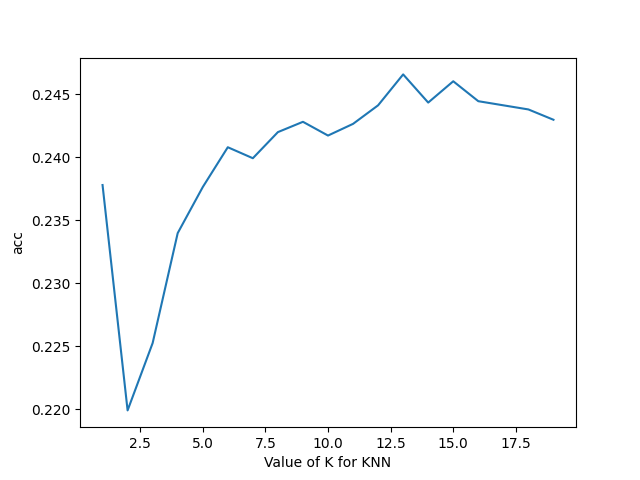
\includegraphics[width=0.4\textwidth]{lateximgs/knn1.png}
    \caption{KNN4SIFT}
\end{figure}

当 $k=13$ 的时候, 使用sift提取特征的knn能够达到平均0.247的正确率. 其次是 $k=15$ 的时候能够到达0.246的正确率. 总的效果并不是很好.
\begin{figure}[h]
    \centering
    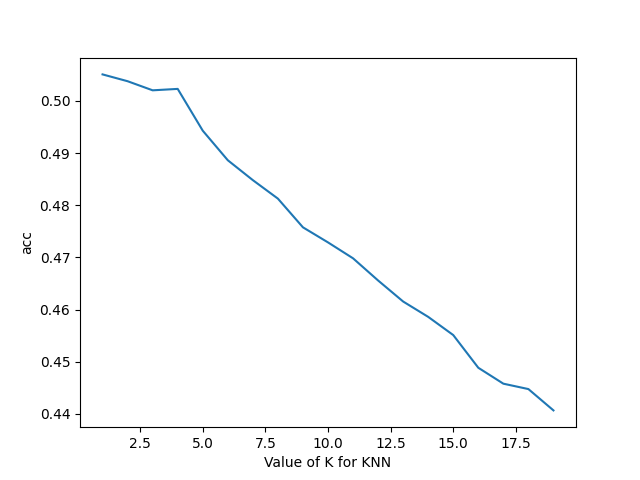
\includegraphics[width=0.4\textwidth]{lateximgs/knn2.png}
    \caption{KNN4HOG}
\end{figure}

对于HOG的情况, 令人震惊的是它竟然在 $k=1$ 的情况最优, acc达到了0.505, 而后面的acc相对于k呈递减趋势, 相比于sift有了巨大进步, 这可能是由于sift特征在转化为单一特征向量的时候经过了聚类和词袋化, 再加上图片本身的特征提取也没有hog那样稳定, 导致转化为特征向量的时候经过了三层的信息损失, 而hog特征提取只经过了pca降维, 导致图片特征保存地较为完全.

\subsubsection{SVM}
支持向量机是传统机器学习内最为著名的分类器之一, 相比于占用内存空间大的KNN, SVM的分类结果仅与支持向量有关, 因此占用内存较小. 在对HOG进行pca降维时可以考虑扩大信息.

在本课设中, 我们采用高斯核, 并设置软间隔参数 $C=1$, 以防止过拟合.

\begin{table}[t]
    \centering
    \begin{tabular}{cccccccc}
    \hline
    model & Fold1 & Fold2 & Fold3 & Fold4 & Fold5 & mean & max\\
    \hline
    svm4sift & 0.352 & 0.320 & 0.321 & 0.345 & 0.328 & $\mathbf{0.333}$ & 0.352\\
    svm4hog & 0.580 & 0.543 & 0.564 & 0.554 & 0.533 & $\mathbf{0.555}$ & 0.580\\
    \hline
    \end{tabular}
    \caption{svm}
\end{table}

上表给出了svm在sift和hog特征上的表现, 可以发现相比于KNN分类器都有较大的提升.

\section{深度学习模型}
\subsection{数据预处理}
\subsubsection{数据增强}
由于深度神经网络极强的拟合能力, 导致其容易对某些不必要的特征过拟合, 因此对图片进行增强是很有必要的, 它能减少模型对某些属性的依赖, 从而提高网络的泛化能力.

由于本课设用到的模型全都是在ImageNet上预训练过的, 因此需要对图像同步在ImageNet上的标准化.

另外由于树叶的特性, 我们可以进行随机翻转、随机旋转等操作. 注意这些操作是在训练的时候对训练集进行的, 这样的话每个epoch的训练集由于数据增强的不确定性会造成不同, 这能够进一步提高模型的泛化能力.
\subsection{模型与参数}
本课设采用了resnet34及其三个变种: resnext50, resnest50和densenet161, 均为预训练模型.
超参数设置如下:
\begin{table}[ht]
    \centering
    \begin{tabular}{ccccc}
    \hline
    Model & Learning rate & Weight decay & Batch size & Num epoch\\
    \hline
    resnet34 & $10^{-4}$ & $10^{-3}$ & 32 & 30\\
    resnext50 & $10^{-3}$ & $10^{-3}$ & 64 & 50\\
    resnest50 & $10^{-4}$ & $10^{-3}$ & 32 & 30\\
    densenet161 & $10^{-4}$ & $10^{-3}$ & 32 & 30\\
    \hline
    \end{tabular}
    \caption{hyper parameters setting}
    \label{tab:example}
    \end{table}
\subsection{Trick}
事实上这部分也可以被认为是数据预处理的范畴, 因为它们是根据跨图片增强的概念提出来的idea, 然而可以通过修改损失函数来实现同样的效果.
\subsubsection{MixUp}
MixUp是一种双图片增强, 在原论文提出的核心公式为:
\begin{equation*}
\begin{aligned}
    \tilde{\bm{x}} &= \lambda \bm{x}_i + (1 - \lambda)\bm{x}_j\\
    \tilde{\bm{y}} &= \lambda \bm{y}_i + (1 - \lambda)\bm{y}_j.
\end{aligned}
\end{equation*}

事实上就是一种双图片按权叠加, 但是可以通过修改损失函数来实现同样效果:
\begin{equation*}
    \mathrm{loss}^{*} = \lambda \mathrm{criterion}_i + (1 - \lambda) \mathrm{criterion}_j.
\end{equation*}

需要注意这里的MixUp同样是在训练的时候进行的, 而不是提前预处理好训练数据.

\subsubsection{CutMix}
CutMix是一种多图片增强, 相比于MixUp在灰度值上的按权叠加, CutMix更为暴力, 它直接在原图片上进行裁剪, 然后将新图片对应的区域直接贴进去.

而对于标签的修改同MixUp. 因此损失函数同样可以写为:
\begin{equation*}
    \mathrm{loss}^{*} = \lambda \mathrm{criterion}_i + (1 - \lambda) \mathrm{criterion}_j.
\end{equation*}

这里 $\lambda$ 为图片i所占新图片的面积占比. 该操作同样在训练中完成.
\subsection{模型效果}
由于该部分没有使用k折交叉验证, 因此对于每一个模型与trick的组合只有一个valid acc数据:
\begin{table}[htbp]
    \centering
    \begin{tabular}{cccc}
    \hline
    Model & Common & MixUp & CutMix\\
    \hline
    resnet34 & 0.943 & 0.942 & $\mathbf{0.951}$\\
    resnext50 & 0.947 & 0.943 & $\mathbf{0.952}$\\
    resnest50 & 0.960 & 0.960 & $\mathbf{0.969}$\\
    densenet161 & 0.959 & 0.956 & $\mathbf{0.965}$\\
    \hline
    \end{tabular}
    \caption{best valid accuracy}
\end{table}

下图是本课设的valid acc曲线:

\begin{figure}[p]
    \centering
    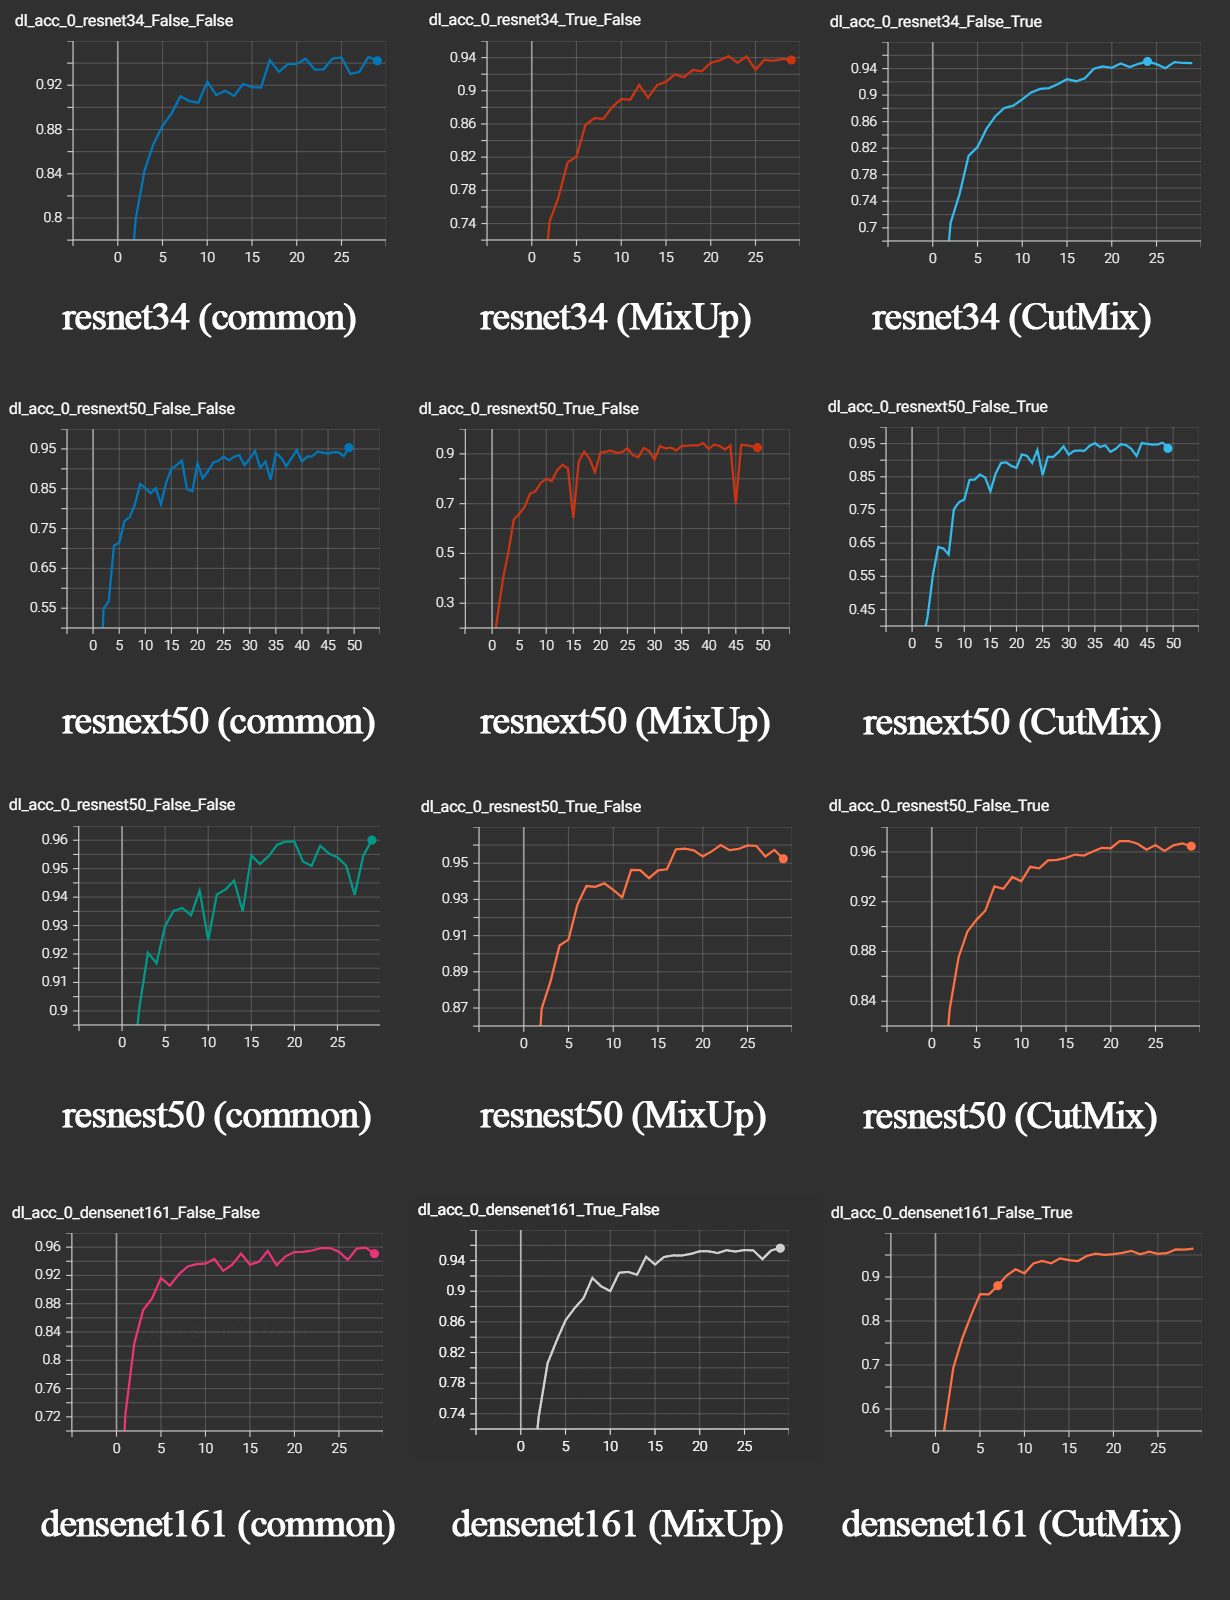
\includegraphics[width=\textwidth]{lateximgs/5.png}
    \caption{valid acc curve (by TensorBoard)}
\end{figure}

\newpage
根据实验结果, 我们发现MixUp trick对于模型精度其实并没有提升, 相反CutMix trick对于模型精度有大约接近0.1的提升. 这可能与树叶的特性有关, 叠加树叶的灰度信息或许并不利于特征提取, 而直接叠加二者的纹理信息可能有助于网络进一步提取特征.

在所有的模型中, resnest50的综合表现最佳, resnext50由于独特的网络设计(以及我故意设的高学习率)导致它的acc曲线较陡, 而即使是最原始的resnet34, 它在验证集上的精度也远高于前面的KNN和SVM分类器在人工提取特征上的效果. 
\end{document}